\subsection{Giao diện thông tin chi tiết workspace}

\begin{figure}[H]
    \centering
    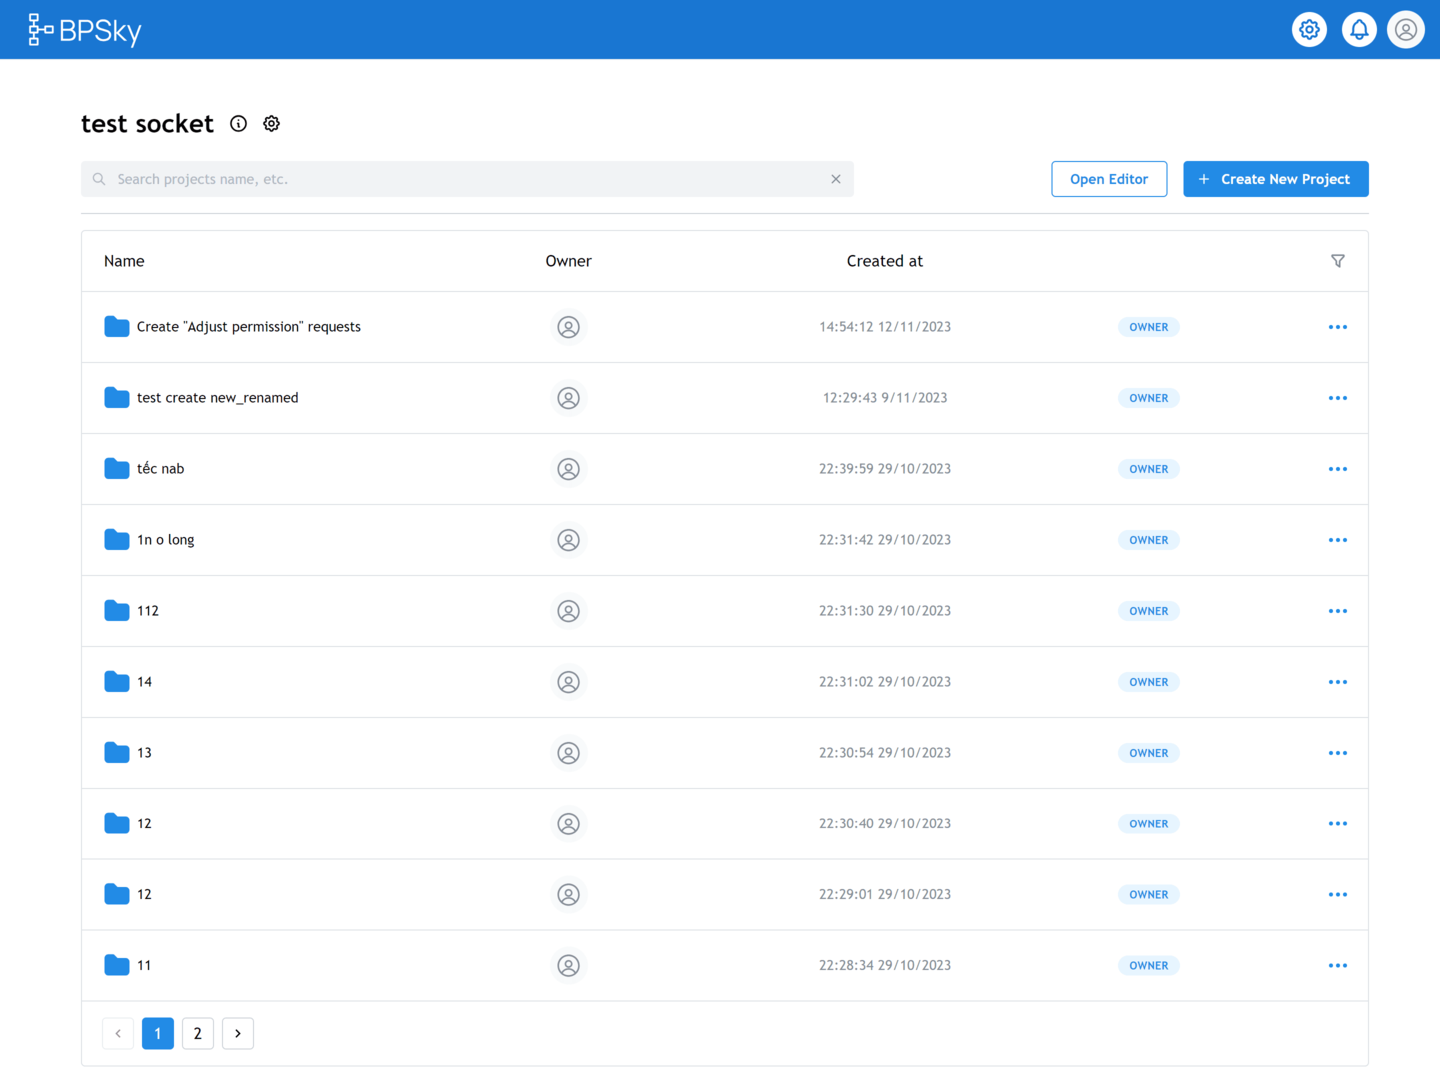
\includegraphics[ width = 0.7\linewidth]{Content/Hiện thực hệ thống/documents/Hiện thực giao diện người dùng/images/WorkspaceDetailPage.png}
    \vspace{0.5cm}
    \caption{Giao diện trang Workspace detail}
    \label{fig: Giao diện trang Workspace detail}
\end{figure}

Người dùng có thể truy cập vào trang Workspace detail bằng cách chọn vào tên của workspace từ danh sách các workspace mà người dùng đang tham gia/sở hữu. Tại đây, người dùng có thể xem danh sách những project có trong workspace. Tương tự với danh sách workspace, mỗi item project cũng sẽ có icon "ba chấm" ở phải cùng, người dùng có thể mở dropdown menu để thao tác với project.